\documentclass[conference]{IEEEtran}
\IEEEoverridecommandlockouts
\usepackage{cite}
\usepackage{amsmath,amssymb}
\usepackage{graphicx}
\usepackage{booktabs}
\usepackage{multirow}
\usepackage{url}
\usepackage{array}
\usepackage{balance}
\graphicspath{{figures/}}

\begin{document}

\title{Card Fraud Triage via Gaussian Mixture Density Scoring: An Unsupervised Anomaly Detection Approach}

\author{\IEEEauthorblockN{Ayush Sahu}
\IEEEauthorblockA{Department of Computer Science and Artificial Intelligence\\
University Name, City, Country\\
Email Address}}

\maketitle

\begin{abstract}
Credit card fraud detection is challenging because fraudulent transactions form a very small fraction of transaction data. This paper investigates an unsupervised anomaly-detection pipeline based on Gaussian Mixture Models (GMMs). The model is fitted only to legitimate training transactions and assigns anomaly scores to validation and test transactions using negative log-likelihood. The experiments use the publicly available European credit-card transaction dataset. After exact-duplicate removal, the data contain 283,726 transactions. A chronological 70/15/15 partition is used, and feature standardization is fitted only on legitimate training observations. The number of Gaussian components is examined from 1 to 40 using information criteria and validation likelihood, followed by repeated-initialization comparisons. A 38-component diagonal-covariance GMM is selected as a practical candidate: it has the lowest AIC and BIC among the tested configurations and a slightly higher mean validation log-likelihood than the 36-component alternative in the repeated $n_{\mathrm{init}}=3$ experiment. At the validation-selected F1 threshold, the final model obtains an Average Precision of 0.2719, precision of 46.94\%, recall of 44.23\%, F1-score of 0.4555, and false-positive rate of 0.0612\% on the evaluated test partition. Operational analyses at fixed false-positive-rate targets and review capacities are also reported. The results establish a reproducible GMM baseline for subsequent fraud-triage research.
\end{abstract}

\begin{IEEEkeywords}
credit card fraud detection, anomaly detection, Gaussian mixture model, unsupervised learning, negative log-likelihood, class imbalance
\end{IEEEkeywords}

\section{Introduction}
Electronic payment systems enable rapid financial transactions but are also exposed to fraudulent activity. Automated fraud detection must identify suspicious transactions while limiting false alarms that consume investigation resources. The task is difficult because fraud is rare, its patterns can change, and labelled examples may not represent future fraud behaviour.

Anomaly detection offers an alternative to directly learning a binary fraud classifier. Instead of fitting a decision boundary using examples of both classes, a normality model is estimated from legitimate transactions. Transactions that receive low probability under this model are ranked as unusual. This study evaluates a Gaussian Mixture Model (GMM) for this purpose. The principal contributions are: (1) a leakage-conscious preprocessing and chronological evaluation pipeline; (2) a component search over 1--40 Gaussian components; (3) a repeated-initialization comparison of candidate component counts; and (4) threshold-based and review-capacity-based evaluation on a highly imbalanced transaction dataset.

\section{Related Work}
Chandola et al. survey anomaly-detection methods and their application domains \cite{chandola2009}. Gaussian mixture models are probabilistic density models commonly estimated using the Expectation-Maximization (EM) procedure. Dempster et al. established the general EM framework for maximum-likelihood estimation with incomplete data \cite{dempster1977}. Information criteria provide complementary approaches to model selection: Akaike introduced AIC \cite{akaike1974}, while Schwarz developed the Bayesian information criterion (BIC) \cite{schwarz1978}. The class-imbalance problem and its implications for machine learning evaluation are discussed by He and Garcia \cite{he2009}. This work uses these established ideas in a normality-modelling pipeline for transaction triage.

\section{Dataset and Exploratory Analysis}
\subsection{Dataset}
The experiments use the European credit-card transaction dataset distributed as \texttt{creditcard.csv} \cite{ulb_dataset}. The original data contain 284,807 records and 31 columns. The columns comprise elapsed time (\texttt{Time}), 28 anonymized PCA-transformed variables (\texttt{V1}--\texttt{V28}), transaction amount (\texttt{Amount}), and the binary class label (\texttt{Class}; 0 for legitimate and 1 for fraud). In the original data, 284,315 transactions are legitimate and 492 are fraudulent.

\subsection{Data quality and class imbalance}
The exploratory analysis found no missing values and identified 1,081 additional occurrences of exact duplicate rows. Exact duplicates were removed. The cleaned dataset contains 283,726 records: 283,253 legitimate and 473 fraudulent transactions. Fraud therefore represents approximately 0.1667\% of the cleaned data. Fig.~\ref{fig:classdist} illustrates the resulting class imbalance. Accuracy alone is consequently not an informative measure of fraud-detection quality.

\begin{figure}[t]
\centering
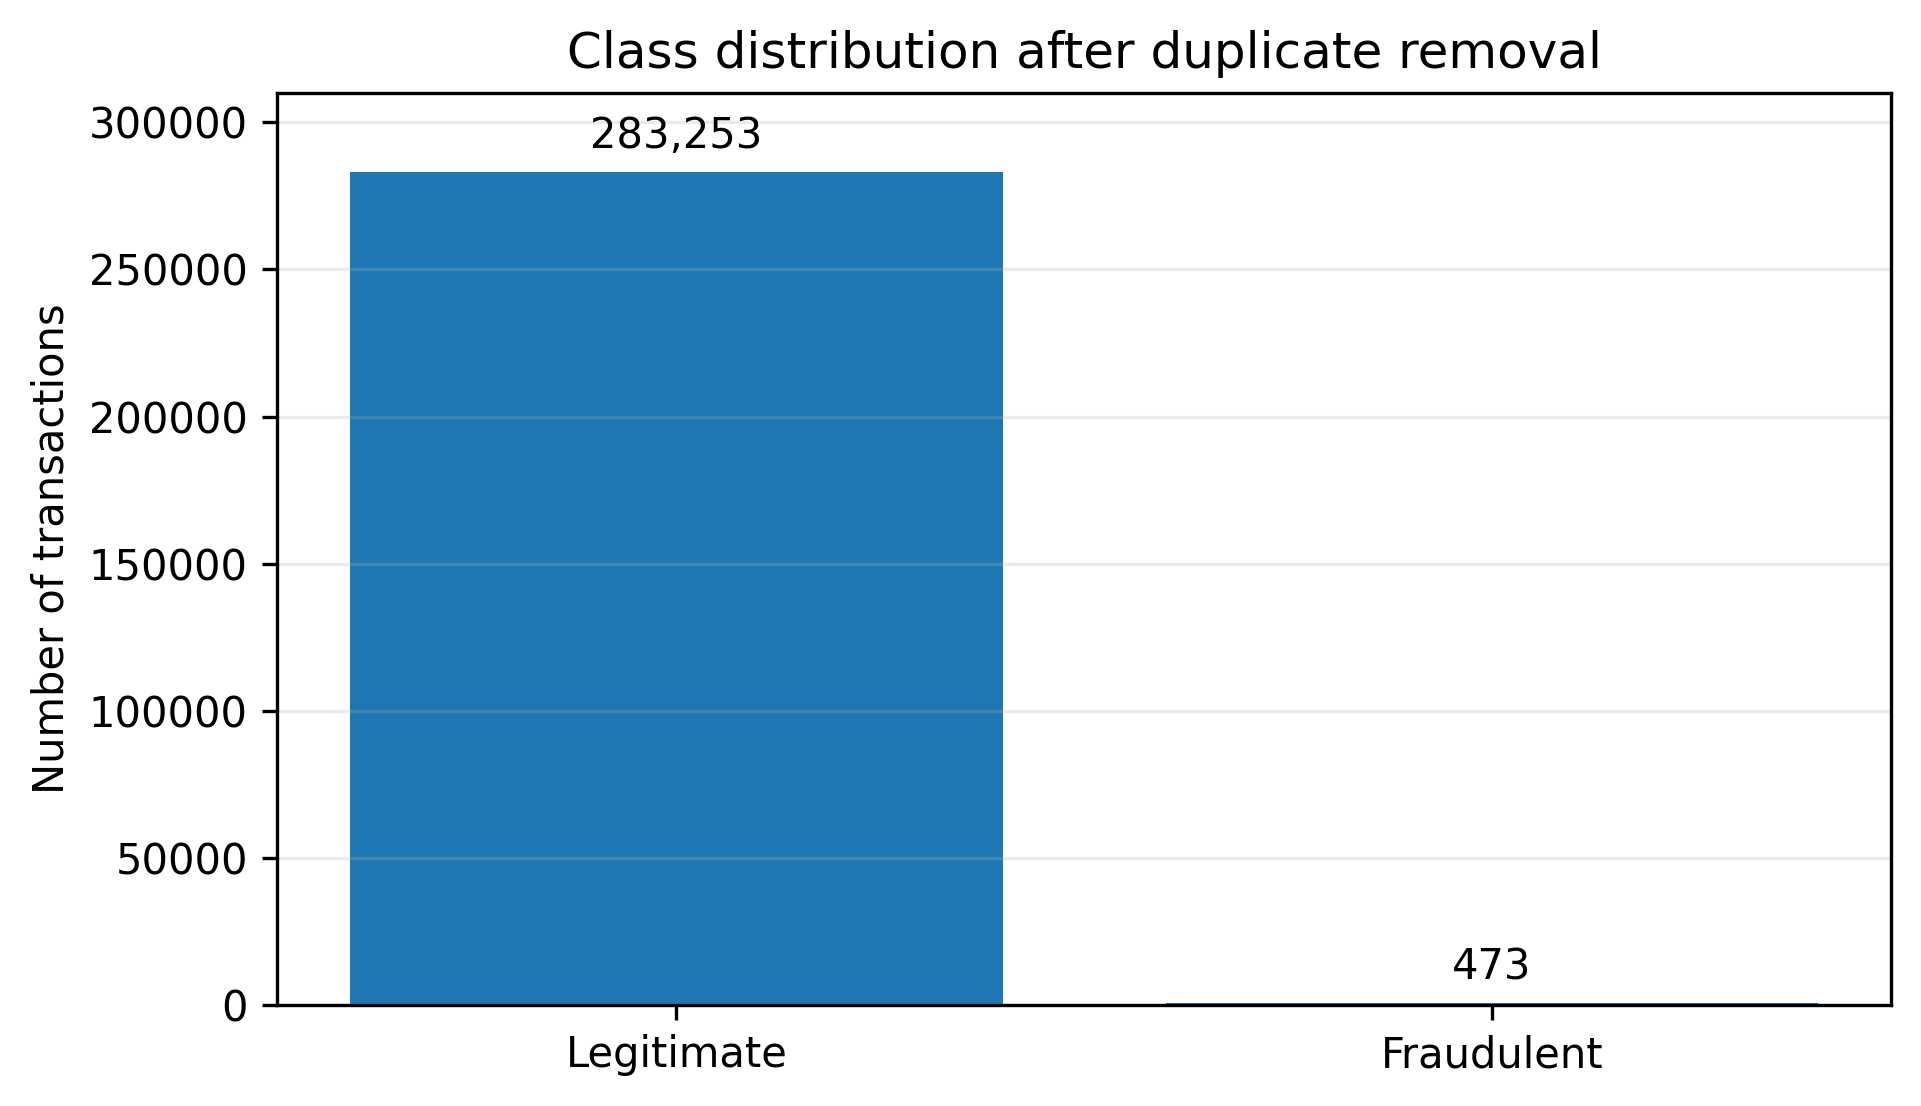
\includegraphics[width=\columnwidth]{class_distribution.png}
\caption{Class distribution after exact-duplicate removal.}
\label{fig:classdist}
\end{figure}

\section{Preprocessing and Experimental Protocol}
\subsection{Chronological partitioning}
The cleaned observations are ordered by \texttt{Time} and divided chronologically into training, validation, and test partitions using a 70/15/15 split. Table~\ref{tab:split} gives the exact partition sizes and class counts. The chronological strategy evaluates later observations after earlier observations rather than randomly mixing transaction order.

\begin{table}[t]
\caption{Chronological data partition after duplicate removal}
\label{tab:split}
\centering
\small
\begin{tabular}{lrrrr}
\toprule
Partition & Total & Legitimate & Fraud & Fraud (\%)\\
\midrule
Training & 198,608 & 198,242 & 366 & 0.1843\\
Validation & 42,559 & 42,504 & 55 & 0.1292\\
Test & 42,559 & 42,507 & 52 & 0.1222\\
\midrule
Total & 283,726 & 283,253 & 473 & 0.1667\\
\bottomrule
\end{tabular}
\end{table}

\subsection{Feature processing}
The class label is excluded from model inputs. The 30 input features are \texttt{Time}, \texttt{V1}--\texttt{V28}, and \texttt{Amount}. A StandardScaler is fitted using only legitimate transactions in the training partition and then applied to validation and test observations. For feature value $x$, standardization is
\begin{equation}
z=\frac{x-\mu_{\mathrm{train,legit}}}{\sigma_{\mathrm{train,legit}}},
\end{equation}
where the mean and standard deviation are estimated only from legitimate training observations. This prevents validation and test data from influencing scaling parameters.

\subsection{Training strategy}
The GMM is fitted exclusively on the 198,242 legitimate training transactions. Fraud labels are not used to estimate the density model. Validation labels are used for model assessment and threshold selection; test labels are used for the reported test evaluation. The cleaned validation and test partitions retain their original class distributions.

\section{Gaussian Mixture Model}
A GMM represents a probability density as a weighted sum of $K$ Gaussian components:
\begin{equation}
p(\mathbf{x})=\sum_{k=1}^{K}\pi_k\,\mathcal{N}(\mathbf{x}\mid\boldsymbol{\mu}_k,\boldsymbol{\Sigma}_k),
\label{eq:gmm}
\end{equation}
where $\pi_k\geq 0$, $\sum_{k=1}^{K}\pi_k=1$, and each component has mean $\boldsymbol{\mu}_k$ and covariance $\boldsymbol{\Sigma}_k$. Model parameters are estimated using EM, which alternates between computing component responsibilities and updating mixture weights, means, and covariance parameters \cite{dempster1977}.

A diagonal covariance structure is used in this study. Each component covariance matrix is constrained to be diagonal, reducing the number of covariance parameters relative to a full covariance model. The model-selection experiment uses the same covariance structure for all candidate values of $K$.

\subsection{Component selection}
The search evaluates $K=1,2,\ldots,40$. AIC and BIC are computed from the fitted training model:
\begin{align}
\mathrm{AIC}&=2p-2\log\hat{L},\\
\mathrm{BIC}&=p\log N-2\log\hat{L},
\end{align}
where $p$ is the number of estimated parameters, $N$ is the number of training observations, and $\hat{L}$ is the maximized likelihood. Lower values are preferred under each criterion. Validation log-likelihood is also recorded for legitimate validation observations.

Fig.~\ref{fig:aicbic} shows the AIC and BIC curves for the 40 tested component counts. Both reach their lowest recorded values at $K=38$. Fig.~\ref{fig:vll} shows that the highest single-run validation log-likelihood occurs at $K=36$, not $K=38$. This distinction is retained in the model-selection rationale.

\begin{figure}[t]
\centering
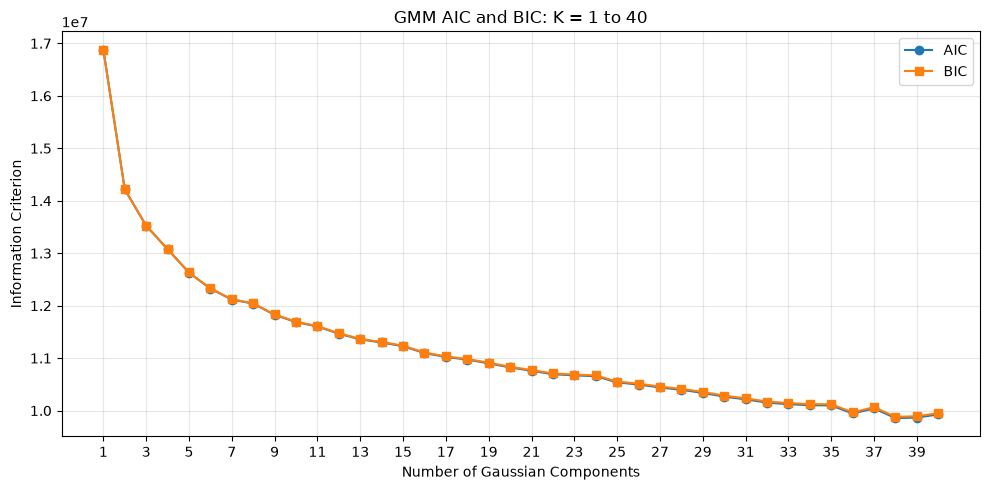
\includegraphics[width=\columnwidth]{aic_bic.png}
\caption{AIC and BIC across the tested GMM component counts ($K=1$--$40$).}
\label{fig:aicbic}
\end{figure}

\begin{figure}[t]
\centering
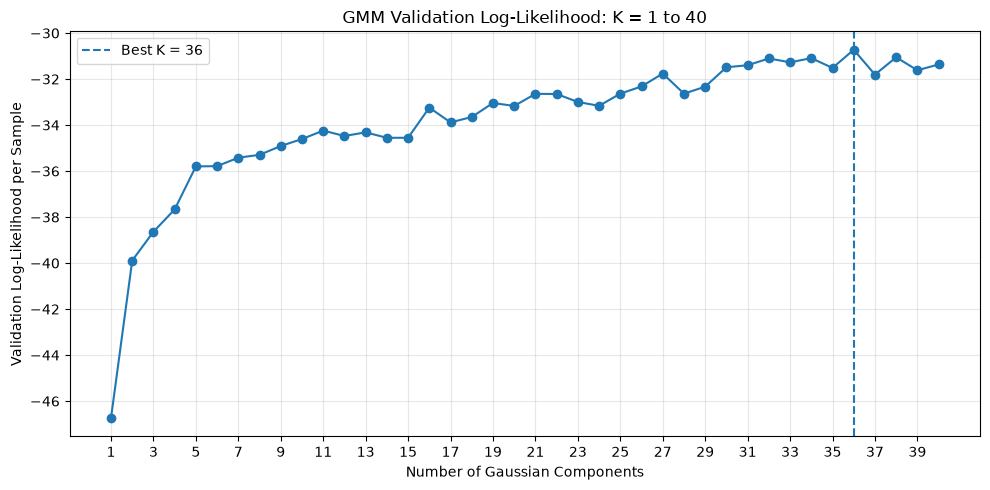
\includegraphics[width=\columnwidth]{validation_log_likelihood.png}
\caption{Legitimate validation log-likelihood across the tested component counts. The best single-run value occurs at $K=36$.}
\label{fig:vll}
\end{figure}

\subsection{Repeated-initialization comparison}
To examine sensitivity to initialization, $K=36$ and $K=38$ are each fitted with five random seeds and $n_{\mathrm{init}}=3$. For $K=36$, mean validation log-likelihood is $-31.4959$ (standard deviation $0.4901$); for $K=38$, it is $-31.4838$ (standard deviation $0.4676$). The paired comparison favours $K=38$ in three of five seeds and $K=36$ in two. The mean difference is small ($0.0121$). Accordingly, $K=38$ is selected as a practical candidate based on the combined AIC/BIC minima and repeated-initialization evidence; it is not claimed to be a globally optimal component count.

\subsection{Anomaly scoring and threshold selection}
For an observation $\mathbf{x}$, the anomaly score is negative log-likelihood:
\begin{equation}
s(\mathbf{x})=-\log p(\mathbf{x}).
\label{eq:score}
\end{equation}
A larger score indicates lower density under the learned legitimate-transaction distribution. An observation is flagged when
\begin{equation}
s(\mathbf{x})\geq\tau,
\end{equation}
where $\tau$ is selected by maximizing F1-score on the validation partition. The final validation-selected threshold is $\tau=94.7575$.

\section{Experimental Results}
\subsection{Implementation}
The pipeline was implemented in Python using Scikit-learn for preprocessing, Gaussian mixture estimation, and metric computation, with Pandas and NumPy for data handling and Matplotlib for plots. The final GMM uses 38 components, diagonal covariance, maximum 200 EM iterations, three initializations, covariance regularization $10^{-5}$, and random state 42. The final fit converged in 111 iterations. Its legitimate validation log-likelihood is $-31.0523$.

\subsection{Test performance}
The test partition contains 42,559 transactions, including 52 fraudulent transactions. At the validation-selected threshold, the final model obtains the metrics in Table~\ref{tab:metrics}. The confusion matrix is shown in Table~\ref{tab:cm}. Average Precision is reported as the summary of the precision-recall curve; the curve is provided in Fig.~\ref{fig:pr}.

\begin{table}[t]
\caption{Final GMM test performance at the validation-selected threshold}
\label{tab:metrics}
\centering
\small
\begin{tabular}{lr}
\toprule
Metric & Result\\
\midrule
Average Precision & 0.2719\\
Precision & 46.94\%\\
Recall & 44.23\%\\
F1-score & 0.4555\\
False-positive rate & 0.0612\%\\
Threshold & 94.7575\\
\bottomrule
\end{tabular}
\end{table}

\begin{table}[t]
\caption{Confusion matrix for the final GMM on the test partition}
\label{tab:cm}
\centering
\small
\begin{tabular}{lrr}
\toprule
 & Predicted legitimate & Predicted fraud\\
\midrule
Actual legitimate & 42,481 & 26\\
Actual fraud & 29 & 23\\
\bottomrule
\end{tabular}
\end{table}

\begin{figure}[t]
\centering
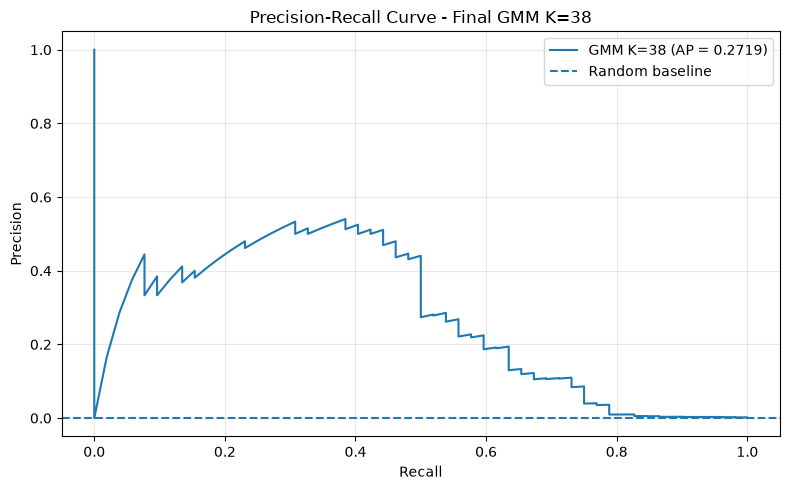
\includegraphics[width=\columnwidth]{precision_recall.png}
\caption{Precision-recall curve for the final $K=38$ GMM on the test partition. Average Precision is 0.2719.}
\label{fig:pr}
\end{figure}

\subsection{Fixed false-positive-rate operation}
For operational analysis, thresholds are determined from legitimate validation anomaly scores at target false-positive rates and then evaluated on the test partition. Table~\ref{tab:fpr} reports the resulting test performance. The observed test false-positive rate need not equal the target exactly because the empirical score distribution is discrete.

\begin{table}[t]
\caption{Final GMM performance at validation-calibrated false-positive-rate targets}
\label{tab:fpr}
\centering
\scriptsize
\begin{tabular}{rrrrr}
\toprule
Target FPR & Test FPR & Recall & Fraud found & False alarms\\
\midrule
1.0\% & 0.743\% & 73.08\% & 38 & 316\\
0.5\% & 0.393\% & 63.46\% & 33 & 167\\
0.1\% & 0.045\% & 40.38\% & 21 & 19\\
\bottomrule
\end{tabular}
\end{table}

\subsection{Limited review capacity}
Transactions are also ranked by anomaly score to simulate a manual-review queue. Table~\ref{tab:topk} shows the number of fraud and legitimate transactions among the highest-scoring observations. At a review capacity of 50, 24 of the selected transactions are fraudulent, giving a precision of 48.00\%.

\begin{table}[t]
\caption{Fraud triage performance at fixed test review capacities}
\label{tab:topk}
\centering
\small
\begin{tabular}{rrrr}
\toprule
Capacity & Fraud found & Legitimate flagged & Precision\\
\midrule
50 & 24 & 26 & 48.00\%\\
100 & 28 & 72 & 28.00\%\\
200 & 33 & 167 & 16.50\%\\
\bottomrule
\end{tabular}
\end{table}

\section{Discussion}
The results show that a GMM trained on legitimate transactions can rank a portion of fraudulent transactions as anomalous. At the selected F1 threshold, 23 of 52 test frauds are detected, while 26 legitimate transactions are incorrectly flagged. The fixed-FPR results show the expected trade-off: allowing a higher false-positive budget increases fraud recall. The top-$K$ results offer a complementary operational view when investigation capacity is constrained.

The model-selection results require careful interpretation. The best single-run validation likelihood is observed at $K=36$, whereas the lowest AIC and BIC values among the tested configurations occur at $K=38$. Repeated initialization gives $K=38$ only a marginally higher mean validation likelihood, and the paired comparison is mixed. Thus, the selected component count is a practical choice supported by several diagnostics rather than a definitive optimum.

\section{Limitations and Threats to Validity}
The diagonal covariance assumption does not model within-component feature correlations. The PCA-transformed input variables also limit direct feature-level interpretation. Further, anomaly detection identifies statistical unusualness rather than proving fraudulent intent; legitimate unusual transactions can be flagged and some fraud may resemble normal behaviour.

An additional evaluation limitation must be disclosed: an earlier $K=11$ baseline was evaluated on the same test partition before the $K=38$ final experiment. Although the component-selection process used validation likelihood and information criteria, prior inspection of test results means the test partition was not a completely untouched one-time holdout throughout the project. The reported $K=38$ test metrics should therefore be interpreted with this exposure in mind. A future study should reserve a new later-period holdout or use a nested temporal evaluation protocol.

\section{Conclusion and Future Work}
This paper presented an unsupervised credit-card fraud-triage pipeline using a diagonal-covariance GMM trained only on legitimate transactions. After duplicate removal and chronological splitting, the final 38-component model achieved Average Precision 0.2719, precision 46.94\%, recall 44.23\%, F1-score 0.4555, and false-positive rate 0.0612\% at the validation-selected threshold. Fixed-FPR and review-capacity analyses further characterized operational trade-offs. These results provide a baseline for the next project phase, which will investigate autoencoder-based anomaly detection and compare it with the GMM approach. A hybrid scoring strategy and a new untouched temporal holdout are also potential directions.

\balance
\begin{thebibliography}{00}
\bibitem{chandola2009} V. Chandola, A. Banerjee, and V. Kumar, ``Anomaly detection: A survey,'' \emph{ACM Computing Surveys}, vol. 41, no. 3, Art. no. 15, 2009.
\bibitem{dempster1977} A. P. Dempster, N. M. Laird, and D. B. Rubin, ``Maximum likelihood from incomplete data via the EM algorithm,'' \emph{Journal of the Royal Statistical Society: Series B (Methodological)}, vol. 39, no. 1, pp. 1--38, 1977.
\bibitem{akaike1974} H. Akaike, ``A new look at the statistical model identification,'' \emph{IEEE Transactions on Automatic Control}, vol. 19, no. 6, pp. 716--723, 1974.
\bibitem{schwarz1978} G. Schwarz, ``Estimating the dimension of a model,'' \emph{The Annals of Statistics}, vol. 6, no. 2, pp. 461--464, 1978.
\bibitem{he2009} H. He and E. A. Garcia, ``Learning from imbalanced data,'' \emph{IEEE Transactions on Knowledge and Data Engineering}, vol. 21, no. 9, pp. 1263--1284, 2009.
\bibitem{ulb_dataset} Machine Learning Group, Universit\'e Libre de Bruxelles, ``Credit Card Fraud Detection dataset,'' publicly distributed through Kaggle. [Online]. Available: \url{https://www.kaggle.com/datasets/mlg-ulb/creditcardfraud}
\end{thebibliography}

\end{document}
